\documentclass{article}
\usepackage{graphicx} % Required for inserting images
\usepackage{amsmath,amssymb}
\usepackage[dvipsnames]{xcolor}
\DeclareRobustCommand{\bbone}{\text{\usefont{U}{bbold}{m}{n}1}}

\DeclareMathOperator{\EX}{\mathbb{E}}% expected value
\title{CS182 Project}
\author{Michael Huang, Chancharik Mitra, Joshua You, Jason Zhang}
\date{March 2023}

\begin{document}

\maketitle

\section{AEs}
\subsection{Autoencoder Warmup}
Let $X \in \mathbb{R}^{nxd}$, $f: \mathbb{R}^{nxd} \to \mathbb{R}^{nxk}$, $g: \mathbb{R}^{nxk} \to \mathbb{R}^{nxd}$. Recall that the optimization problem we solve for autoencoders were:
\begin{equation}
    \arg\min_{f, g} ||X - g(f(X))||_F^2
\end{equation}
\textbf{What do the functions $f$ and $g$ represent here? How can we learn $f$ and $g$?}
\\
\section{VAEs} 
VAEs, or (V)ariational (A)uto(e)ncoders are a special type of autoencoder that generates new outputs rather than just output lower dimensionality data we've already seen before. More generally, VAEs generate \textit{new} information given patterns we've seen about the data. To do this, we'll need some probability theory under our belt.
\subsection{On the Loss Function of VAEs}
\begin{enumerate}
    \item Recall in autoencoders, we have an encoder to decoder structure with a bottleneck in between. We can denote the learning parameters for the encoder as $\phi$ and the decoder as $\theta$, and $z$ as our latent representation. The variational autoencoder has the same principles, but we now fit a probability distribution over the encoder decoder structure to generate new samples.
    \\
    \\
    More formally, we create a \textit{probabilistic encoder} and fit a probability distribution $q_{\phi}(z|x)$ to generate latent representations $z$, then fit a \textit{probabilistic decoder} and fit a probability distribution $p_{\theta}(x|z)$. The true goal of using these distributions is to sample $z \sim q_{\phi}(z|x)$ and use $z$ to generate new $x' \sim p_{\theta}(x|z)$. (Intuition Goes Here)
    \\
    \\
    Let's try to further our understanding of why we do this intuitively. Suppose we have a hidden latent random variable $Z$ that affects a seen random variable $X$. \textbf{Given observations of $X$, (i.e we have $p(x|z)$), explain why it's difficult to find $p(z|x)$.}
    \\
    \textit{hint: Recall that the definition of conditional probability is that: 
    $$p(z|x) = \frac{p(z, x)}{p(x)} = \frac{p(x | z)p(z)}{p(x)}$$}
    \item Instead of trying to find $p(z|x)$ to generate new samples $x'$, we can instead try to find a distribution $q(z|x)$ that is as close to $p(z|x)$ as possible that has a \textit{tractable} solution. One way can measure the distance between probability distributions is to use something know as the \textit{Kullback-Leibler Divergence}, which is defined to be $D_{KL}(p||q) = \EX_p[\log(\frac{p(X)}{q(X)})]$. From an information theory perspective, it measures the relative entropy from using $q$ as a model when the actual distribution is $p$. \textbf{Show that by using the KL divergence, we can rewrite the minimization problem $D_{KL}(q_{\phi}(z|x) || p_{\theta}(z|x))$} as:
    $$\arg\max_{\theta, \phi}\EX_{q_{\phi}(z|x)}[\log(p(x|z))] - D_{KL}(q_{\phi}(z|x) || p_{\theta}(z))$$
    rewriting this expression gives us 
    $$\arg\min_{\theta, \phi} D_{KL}(q_{\phi}(z|x) || p_{\theta}(z)) - \EX_{q_{\phi}(z|x)}[\log(p_{\theta}(x|z))]$$
    \textbf{Intuitively speaking, what does $-\EX_{q_{\phi}(z|x)}[\log(p_{\theta}(x|z))]$ represent?}
    \textit{hint 1: Start with the definition of KL Divergence, and remove terms that are irrelavant to the minimization problem.}
    \\
    \textit{hint 2: Recall that we draw a sample $z$, and use that to reconstruct $x'$ What does it mean then to maximize the log probability of our training set when reconstructing $x'$?}
\end{enumerate}
\newpage
\subsection{Modeling VAEs using Gausssians and The Reparameritization Trick}
We definitely don't know the distribution of our data at first glance, but one surefire method that works well in machine learning is \textbf{to model everything as a Gaussian}. In other words, we model $p(z) \sim N(0, I)$ and $p(x|z) \sim N(f(z), cI)$, where $f$ isn't known to us \textit{yet}. We say the mean is $f(z)$ because we're not sure how the distribution will shift given the latent variable. Recall that $q(z|x)$ is an approximation of $p(z|x)$, which was intractable to find. Thus, \textit{the next best thing is to model it as a flexible normal}, i.e $q(z|x) \sim N(g(x), h(x))$, where $g$ and $h$ are not known yet.
\begin{enumerate}
    \item Recall that the loss function for VAEs were:
    \begin{equation}
        D_{KL}(q(z|x) || p(z)) - \EX_{q(z|x)}[\log(p(x|z))]
    \end{equation}
    \textbf{Show that we can minimize (1) as:}
    \begin{equation}
        \arg\min_{f, g, h} \EX_{q(z|x)}[||x - f(z)||_2^2] + \lambda D_{KL}(q(z|x) || p(z))]
    \end{equation}
    \textbf{Where $\lambda$ is a term you derive. Does this look similar to the autoencoder loss function? What would $f, g, h$ represent in the vanilla autoencoder structure?}

    \item $f$, $g$, and $h$ are all learnable functions that can all be trained using the neural network architectures that we've learned in class. However, with the way VAEs work, our backpropagation pipeline is seperated because we are sampling $z$ from $q(z|x)$, so there are no derivatives that can flow back to the encoder. Luckily, researchers came up with the \textit{Reaper Reparameterization Trick}. Instead of sampling directly from $z \sim N(f(x), g(x))$, we instead say $z = \_\_\_ + \_\_\_ * Z$, where $Z \sim N(0, I)$. \textbf{Fill in the blanks, and explain how this allows derivatives to flow back to the encoder through backpropagation}.

    \item Now you'll try it for yourself! We will create a Variational Autoencoder using Pytorch to generate digits from the MNIST dataset, then use the VAE to train a convolutional neural network to classify digits to see how well it can retain information.
\end{enumerate}

\subsection{An alternative formulation}


\section{VQ-VAEs}
Recall that there are three steps when it comes to Variational Auto Encoders:
\begin{enumerate}
    \item Make our encoder \textit{random} by giving it an input $x$, sample from seeing $x$, and try to reconstruct $x$
    \item Add a regularizer during training that tries to keep our latent distribution close to where we want to sample from (i.e keep our latent distribution close to $N(0, I)$)
    \item Train using the Reaper Reparameterization Trick.
\end{enumerate}
However, VAEs suffer from a phenomenon known as \textit{posterior collapse}, meaning that the decoder starts ignoring the latent distribution, forcing the decoder the create generic outputs. In image generation, this is possibly due to the fact that images are naturally drawn from a discrete distribution rather than a continuous distribution, so the our sampling codes (i.e a standard normal) may not be able to learn the signals from our training data $x$ resulting in posterior collapse. To mitigate this, we use the VQ-VAE (Vector Quantitized Variational AutoEncoder). Instead of using contionious latent codes, the VQ-VAE using discrete latent codes to generate images. In this problem, we build the VQ-VAE together.
\subsection{On the VQ-VAE Architecture}
Everything about the VQ-VAE architecture and the VAE architecture is the same except for the latent distribution. Instead of sampling from a continious distribution to generate randomness, we now sample from a discrete distribution. We can do this by introducing a set of vector embeddings (the number of vectors is a number we choose) that will represent our discrete distribution. Figure 1 represents this.
\begin{figure}[h]
    \centering
    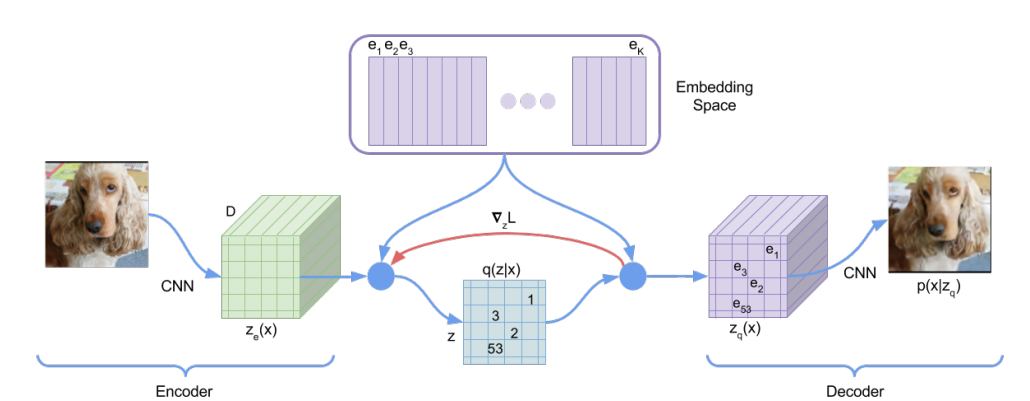
\includegraphics[width=1.0\textwidth]{image.png}
    \caption{The VQ-VAE Architecture}
    \label{fig:mesh1}
\end{figure}
\newline
Suppose we can decompose an image $x$ into $n$ different latent vectors (i.e we use a convolutional encoder). \textbf{Give one way we can sample the encoding space by using the $n$ latent vectors from our encoding}.
\newpage
\subsection{Training VQ-VAEs}
\begin{enumerate}
    \item Recall that the loss function for VAEs was defined as:
$$\arg\min_{\theta, \phi} D_{KL}(q_{\phi}(z|x) || p_{\theta}(z)) - \EX[log(q_{\phi}(x|z))]$$
Where $\EX[log(q_{\phi}(x|z))]$ is our reconstruction loss, and $D_{KL}(q_{\phi}(z|x) || p_{\theta}(z))$ is our regularizer to keep it our latent distribution close to what we want to sample from. However, there is a problem with simply reflecting this loss function with the VQ-VAE.
\\
\\
As with before, since we are sampling from the discrete embedding space, none of our gradients will backpropogate to the decoder. We can't use the reparameterization trick, because we don't actually know the discrete distribution, we are just fitting it. One method researchers have used to combat this is to simply copy the gradients from the decoder to the encoder. \textbf{Let $\tilde{x}$ be our latent output from the encoder, and let $\hat{x}$ be the sampled input to the decoder. Furthermore, let the stop gradient function $sg(x)$ represent a function that blocks gradients to backpropagate through. Define $\hat{x}$ in a way that allows the decoder gradients to be copied over to the encoder using $\hat{x}, \tilde{x}, $ and the stopgradient function $sg(x)$.}

\item The way we are sampling from the discrete distribution does not allow gradients to update the distribution itself. Ideally, the encoding of $x$ represents its latent sampling, so we would like our distribution to represent the latent samples we get from the encoder. \textbf{Using the stop gradient function $sg$, our sampled encodings from our distribution $e$, and our encoded data $z_e(x)$, provide a term that will allow our sampled encodings to update to be closer to our encoder outputs.}

\item Another problem is that our encoder output can grow arbitrarily and not fit to the discrete encoding distribution we create. Thus, we should add a committment loss term that keeps the encoder committed to the latent encoding distribution. \textbf{Using the stop gradient function $sg$, our sampled encodings from our distribution $e$, and our encoded data $z_e(x)$, provide a term that will allow our encoder to update to be closer to our sampled encodings.}

\item After we've trained a VQ-VAE to encode and decode images, we are left with encodings from our discrete latent distribution that is able to create images from the CIFAR-10 distribution. However, we don't have an immediate way to generate an image from CIFAR-10 because we don't know the distributions of the encodings, just the patterns themselves. \textbf{Given the latent distribution samples, give one way we can generate latent distribution samples so that we can generate images from the CIFAR-10 dataset.}
\end{enumerate}

\end{document}
